\section{PDF Implementierung}
PDF ist eine vektorbasierte \gls{pdl} (Seitenbeschreibungssprache) und basiert auf dem PostScript-Format. Der \gls{mime} Type von PDF heißt application/pdf. Eine \gls{pdl} beschreibt den Seitenaufbau, wie die Seite in einem Ausgabeprogramm bzw. Ausgabegerät, z.B. einem Drucker, aussehen soll. \gls{pdl}s können Seiten mit Vektoren beschreiben. An den Drucker wird durch die \gls{pdl} ein Datenstrom der zu druckenden Ausgabe erzeugt und an den Drucker gesendet. Der \gls{rip} eines Druckers wandelt die Bildschirmausgabe in die gerasterte Druckerausgabe um. Viele \gls{api}s der Hardwareabstraktionsschicht im Computer wie \gls{gdi} oder OpenGL können in \gls{pdl} ausgeben. Speichert ein Satzprogramm den Seitenbeschreibungscode eines Dokuments in einer Datei, müssen Drucker die \gls{pdl} nicht selbst verarbeiten. Eine \gls{ppd} Druckerbeschreibungsdatei definiert Fonts, Papiergröße, Auflösung und andere Standardeigenschaften für einen bestimmten PostScript-Drucker \cite{ppd-file}. Im Common Unix Printing System, der Standard-Druckersteuerung von Linux hat der PostScript und der PDF-Interpreter ghostscript die Aufgabe eines \gls{rip}, d.h. er ist für die Umwandlung in die gerasterte Druckausgabe auf dem Drucker zuständig. Zudem stellen \gls{pdl}s eine Schnittstelle zum Quellcode eines Dokuments bzw. zu Programmen, die Quellcode verwalten oder das Dokument formatieren können, dar. Die \gls{pdl} PDF erweitert die Funktionalität von PostScript um anklickbare Links (Hypertextfunktionalität), die die Navigation im Dokument erleichtern und URLs, die sich automatisch im Browser öffnen \cite{wiki-pdl}.

\subsection{PostScript}
Sowohl die PostScript als auch PDF haben zum Ziel die Seiten eines Dokuments vollständig für die Ausgabe in der Druckvorstufe zu beschreiben. Die abwärtskompatible, stackorientierte, Turning-vollständige Hochsprache PostScript als \gls{pdl} wurde in den 1980er Jahren von Adobe erfunden \cite{adobe-postscript, wiki-postscript}. Hinzu wurden weitere PostScript-Technologien entwickelt, die aus der Programmiersprache PostScript, Grafik-, Textformatierungsanwendungen, Treibern und Abbildungssystemen bestehen. PostScript hat sich als Industriestandard etabliert. Die letzte Version ist PostScript 3 von 1997. Seine primäre Anwendung gemäß des Adobe Imaging Models findet sich in der Beschreibung von Textdarstellung, graphische Formen und Bildern auf gedruckten oder auf dem Bildschirm angezeigten Seiten. Dabei ist die Beschreibung des Dokuments geräteunabhängig und eine PostScript-Datei ist sequentiell organisiert. PostScript unterstützt u.a. beliebige geometrische Formen, Zeichenoperationen in Graustufen, RGB, CMYK und CIE (Yxy-Farbraum), vorinstallierte oder benutzerdefinierte Fonts, Digitalbilder jeglicher Auflösung, je nach Farbmodell, und ein allgemeines Koordinatensystem. \\
In PostScript wird eine Seite, die ein Koordinatensystem umspannt, als Grafik betrachtet, die verschiedene Grafikelemente enthalten kann. Dabei werden die Textzeichen eines Fonts, gemäß des Adobe Imaging Models, als graphische Formen betrachtet auf denen Grafikoperationen möglich sind. Das Koordinatensystem unterstützt alle linearen Transformationen, die auf jegliche Seitenelemente angewendet werden können. Die Seitenbeschreibung in PostScript kann auf jedem Gerät, was einen PostScript-Interpreter implementiert, gerendert werden. In diesem Prozess wird die high-level PostScript-Beschreibung in low-level Rasterdatenformate für das jeweilige Gerät übersetzt. Jede PostScript-Datei muss durch einen \gls{rip} interpretiert und die Dateien können in \gls{ascii} vorliegen \cite{adobe-postscript}. Der PostScript-Interpreter als \gls{rip} rechnet die Benutzerkoordinaten in Gerätepixel um, wobei auch die technischen Eckdaten des jeweiligen Geräts mitberücksichtigt werden. Theoretisch kann derselbe PostScript-Code auf verschiedenen Endgeräten mit unterschiedlicher Auflösung eine mehr oder weniger identische Ausgaben erreichen. Den Interpreter gab es früher als Hardware-\gls{rip}, der allerdings nicht mehr zum Einsatz kommt. Heute gibt es lediglich Software-\gls{rip}s, die von einem Betriebssystem kontrolliert werden und hardwareunabhängig arbeiten. Fast alle \gls{rip}-Hersteller orientieren sich am Standard und somit sind PostScript-Fehler in der Druckvorstufe minimiert worden \cite{schneeberger}.

\subsection{Adobe Imaging Model}
PDF und die PostScript Programmiersprache haben das Adobe Imaging Model als Gemeinsamkeit. Es kann nahtlos zwischen PDF und PostScript konvertiert werden und beide erzielen das gleiche Ausgabeergebnis beim Druck. Dennoch fehlt PDF das general-purpose Framework der PostScript Programmiersprache. Stattdessen stellt ein PDF Dokument eine statische Datenstruktur optimiert für den random-access auf beliebigen Seiten dar und enthält zusätzlich Seitennavigationsinformationen für interaktives Lesen. Im Kontrast dazu sind PostScript-Dateien seriell organisiert. \\
Das high-level Imaging Model beschreibt die Elemente, die auf der Seite dargestellt werden, also Text, Geometrie oder Vektorgrafiken, als abstrakte graphische Elemente aus Vektorobjekten und Bézierkurven, anstatt als Pixeldefinitionen. Pfad-Objekte werden durch verbundenen Punkten, Linien und Kurven mathematisch berechnet. Text-Objekte bilden eine eigene Datenstruktur (Fonts), die als Glyphen aus Pfad-Objekten bestehen. Bild-Objekte sind aus einzelnen Pixelwerten in einer rechteckigen Fläche aufgebaut und enthalten eine eindeutige Position im Rechteck und einen Farbwert. Die abstrakte Beschreibung graphischer Elemente macht das Imaging Model zu einem geräteunabhängigen Modell und es kann hochwertige Ausgaben auf vielen verschiedenen Druckern und Bildschirmen liefern. \\
Eine Anwendung generiert zuerst die geräteunabhängige Beschreibung des gewünschten Ausgabegeräts in der \gls{pdl}. Daraufhin interpretiert eine Firmware oder Software eines spezifischen Ausgabegeräts für Rasterausgaben die Beschreibung und rendert sie im Ausgabegerät. Hierbei hat die \gls{pdl} die Rolle eines Austauschstandards für die Übertragung und Speicherung von druckbaren oder auf Displays darstellbaren Dokumenten \cite{adobe-postscript}. Die Flexibilität des Adobe Imaging Models zeichnet sich durch seine flexible Ausgabefähigkeit auf jeglichen Rastergeräten und hochauflösenden Displays. Die Größe des Pixels wird durch die Ausgabeauflösung des Rastergeräts bestimmt, die bei Monitoren zwischen 75 und 110 \gls{ppi} und bei Tintentstrahl- bzw. Laserdruckern zwischen 300 und 1400 \gls{ppi} liegt. \\
Später wurde das Imaging Model für die Unterstützung von Transparenzen erweitert. Diese Funktionalität wurde speziell für PDF implementiert und wird nicht von PostScript unterstützt. Bei PostScript überschreibt das zuletzt gezeichnete Objekt alle darunterliegenden Objekte im Hintergrund \cite{schneeberger}. 

\subsection{Dateiformataufbau}
PDF ist ein reines objektbasiertes Dateiformat und PDF-Dateien enthalten Dokumentdaten in binärer Form. PDF-Dateien bestehen aus Sequenzen von 8-Bit-Binärdaten bzw. 7-Bit-\gls{ascii} \cite{schneeberger}. Ein Dokument entspricht immer einer Datei. Das Einbetten von binären Dateien in beliebigen Formaten oder anderer PDF-Dateien ist möglich. Die Struktur besteht im Wesentlichen aus 4 Komponenten. Zunächst spezifiziert der Header die Version der PDF-Spezifikation (signature) und den Charset Identifier \cite{ccc-pdf-secrets}. Zwei Beispiele eines Headers sind in den Abbildungen \ref{fig:header1} und \ref{fig:header2} gezeigt. Der Body enthält die Daten der Objekte, aus denen das Dokument besteht. Objekte im Body sind in einer komplizierten hierarchischen Struktur, dem Dokument, verknüpft. Zur Dateigrößenoptimierung werden komplexe Verbindungen zwischen den Daten hergestellt und die Daten eines mehrfach vorkommenden Objektes müssen nur einmal gespeichert werden \cite{softx}. Jedes Objekt wird im Body mit obj und endobject eingekapselt und jeder Stream mit stream und endstream \cite{schneeberger}. Eine Beispielabbildung \ref{fig:body} ist weiter unten zu sehen. Die Cross-Reference Table (Xref) deckt die Informationen über die Position der indirekten Objekte in der Datei ab. Liegt ein Verweis auf ein Objekt in der Xref, so kann es für andere Seiten wiederverwendet werden. In Xref sind alle Informationen für den random-access eingetragen. Neben Objekteinträgen können auch Cross-Reference-Streams hinterlegt werden. Xref ist der einzige Teil in PDF mit einem konstanten Format und kann aus mehreren Cross-Reference-Sections und Subsections jeweils mit Objekteinträgen für das incremental update bestehen. Ein Objekteintrag ist wie folgt aufgebaut: Die ersten 10 Bytes für die Byteposition (Offset), mit Leerzeichen als 1 Byte getrennt, die folgenden 5 Bytes für die eindeutige Generation Number und zuletzt eine ebenfalls durch ein Leerzeichen getrennte Markierung mit f oder n. f steht für free entry, d.h. gelöschtes Objekt, und n für in use entry. Das erste Objekt in Xref hat eine generation number von 0 und wird nicht verwendet. Eine beispielhafte Xref ist in einer Abbildung \ref{fig:xref} gezeigt. Zuletzt definiert der Trailer die Startposition der Cross-Reference Table als Pointer startxref und von speziellen Objekten im Body \cite{ccc-break-pdf}.  Außerdem enthält der Trailer die ID der PDF-Datei, einen Size Entry, Metadaten und eine Referenz zum /Root Objekt (Katalog) im Body. Abschließend markiert \%\%EOF das Dateiende \cite{ccc-break-pdf, ccc-pdf-secrets}. Zwei Trailerbeispiele sind in Abbildungen \ref{fig:trailer1} und \ref{fig:trailer2} dargestellt.

\begin{figure}[!htb]
	\centering
	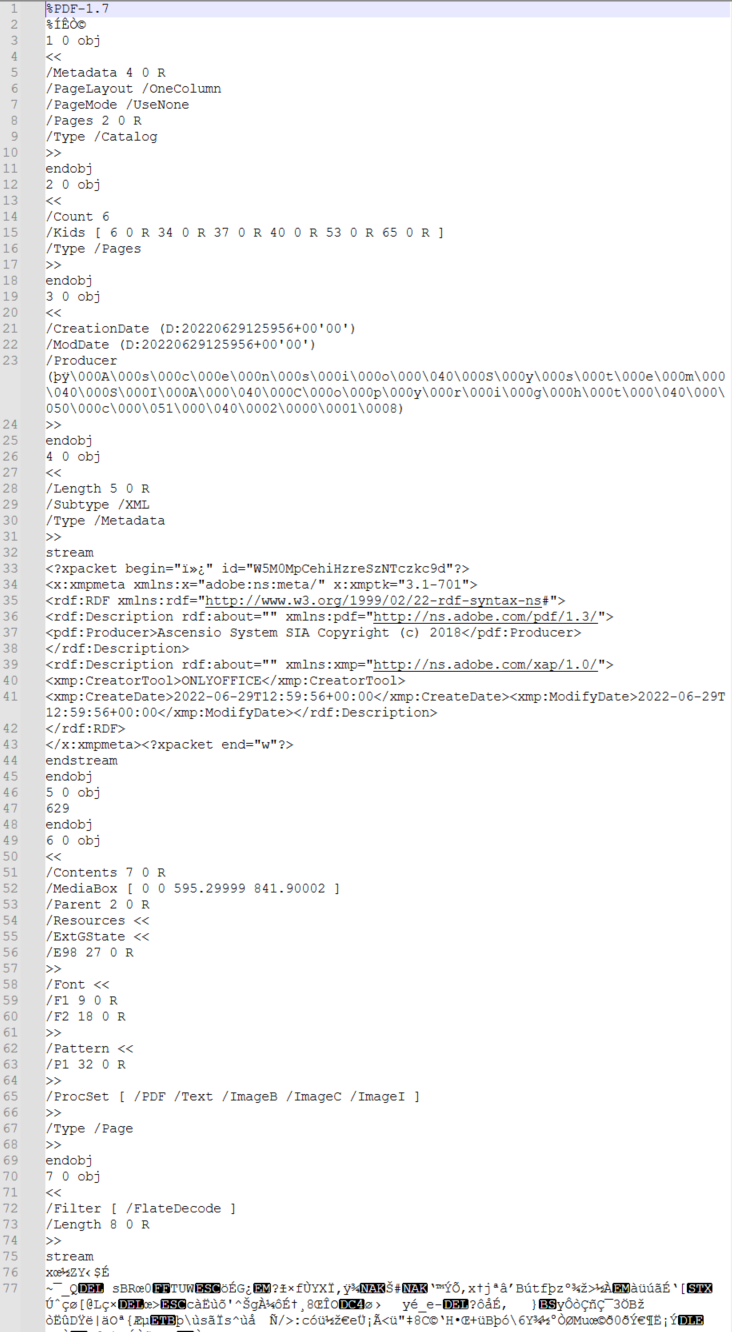
\includegraphics[width=0.8\textwidth]{"images/pdf_header2-notepad.png"}
	\caption{Header und Beginn eines Bodys des PDF-Dateiformats in Notepad++}
	\label{fig:header1}
\end{figure}

\begin{figure}[!htb]
	\centering
	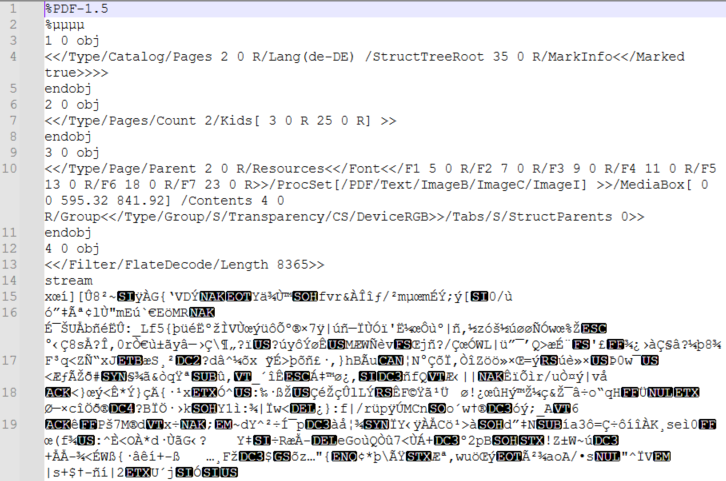
\includegraphics[width=0.8\textwidth]{"images/pdf_header-notepad.png"}
	\caption{Header, Beginn eines Bodys mit Katalog und Binärdaten des PDF-Dateiformats in Notepad++}
	\label{fig:header2}
\end{figure}

\begin{figure}[!htb]
	\centering
	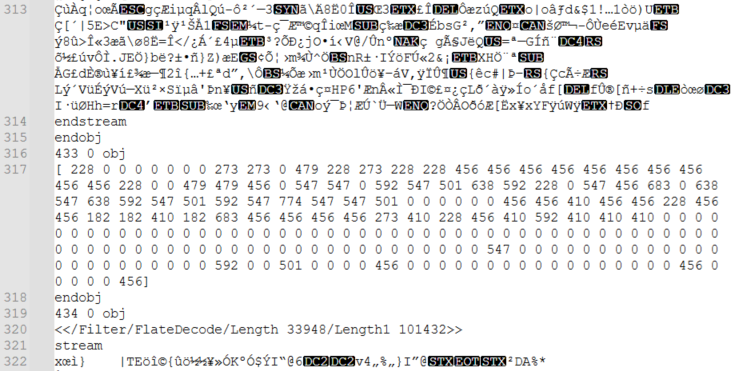
\includegraphics[width=0.8\textwidth]{"images/pdf_body2-notepad.png"}
	\caption{PDF Bodyauszug des PDF-Dateiformats in Notepad++}
	\label{fig:body}
\end{figure}

\begin{figure}[!htb]
	\centering
	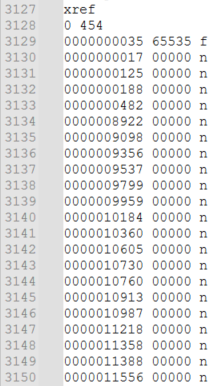
\includegraphics[width=0.5\textwidth]{"images/pdf_xref_start-notepad.png"}
	\caption{PDF Xref des PDF-Dateiformats in Notepad++}
	\label{fig:xref}
\end{figure}

\begin{figure}[!htb]
	\centering
	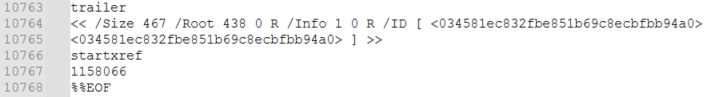
\includegraphics[width=0.8\textwidth]{"images/pdf_trailer-notepad.png"}
	\caption{Kurzer Trailer des PDF-Dateiformats in Notepad++}
	\label{fig:trailer1}
\end{figure}

\begin{figure}[!htb]
	\centering
	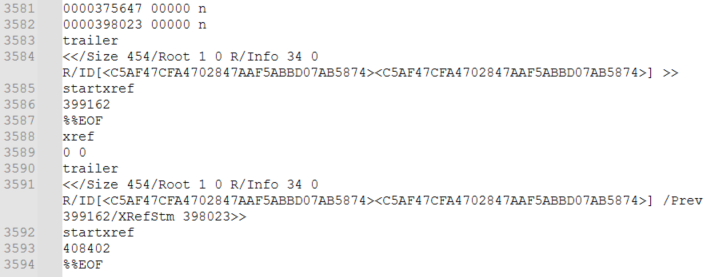
\includegraphics[width=0.8\textwidth]{"images/pdf_trailer2-notepad.png"}
	\caption{Ende einer Xref und Trailer des PDF-Dateiformats in Notepad++}
	\label{fig:trailer2}
\end{figure}

Beim incremental update wird am Ende der Original-Trailers ein Body-Update, eine neue Xref-Section und ein updated Trailer der Datei hinzugefügt. In der neuen Version der Xref-Section werden alle Objekte aufgeführt, die gelöscht, geändert oder ersetzt wurden. Der Updated Trailer umfasst alle Änderungen bezüglich des originalen Trailers \cite{schneeberger}. PDF-Viewer prozessieren PDF-Dateien im Prinzip vom Ende bis zum Anfang, d.h. vom Trailer zum Body \cite{ccc-break-pdf}. Beim Parsen wird zunächst die signature überprüft, dann wird die Position von \%\%EOF und startxref gesucht, was die Position der Xref angibt. Die Xref stellt die Offsets jedes Objektes zur Verfügung und der Trailer zeigt auf den /Root Entry des Root-Objekts. Nachfolgend werden alle Objekte geparst und überprüft, ob /Root den /Pages Entry, /Pages ein Seiten-Array, jede /Page eine Größe der /MediaBox hat, /Contents als Stream-Objekt vorliegt und /Resources das /Font dictionary definiert. Zuletzt wird die Seite gerendert durch BeginText, Auswahl des Fonts, Bewegung des Cursors, Anzeigen des Strings und EndText \cite{ccc-pdf-secrets}. Referenzen werden nicht in der parse time ausgewertet, sondern nur nach Verwendung \cite{ccc-wtf-pdf}.
\par
Seitenobjekte und die meisten PDF-Strukturen sind gerichtete azyklische Graphen \cite{ccc-wtf-pdf}. PDF-Objekte können in den folgenden Typen vorliegen: Booleans, Integers oder reelle Zahlen, Strings, Namen, die mit einem / Zeichen beginnen, Arrays, Dictionaries, Streams, Null-Objekt oder Kommentare mit einem vorangestellten \%. Strings können als <Length> <string> oder <string> <terminating symbol> definiert werden. Dictionary Objekte sind als ein Paar von Objekten, genannt Entries, implementiert. Aktionen werden beispielsweise als Entries gespeichert \cite{ccc-badpdf}. \\
Text in AcroForms wird als Stream gespeichert. In Streams kann alles gespeichert werden und sie werden nicht interpretiert. Die Objekte in Streams können Referenzen auf andere Objekte vor allem Seiten enthalten \cite{ccc-break-pdf}. Objekte können so gruppiert werden, wodurch eine bessere Komprimierung erreicht wird, vor allem bei der Gruppierung von Linien \cite{schneeberger}. \\
Es gibt graphics state-Operatoren, die eine Datenstruktur, genannt graphics state, manipulieren. Graphics state ist ein globales Framework mit dem andere Grafikoperatoren ausgeführt werden. Es enthält die aktuelle Transformationsmatrix (CTM), welche die Benutzerortskoordinaten in Ausgabegerätekoordinaten mappt, die aktuelle Farbe, den aktuellen Clipping-Pfad und andere Parameter, die implizite Operanden von Zeichenoperatoren sind. Außerdem gibt es noch Pfaderstellungsoperatoren, Pfadzeichenoperatoren und Textoperatoren. Zusätzlich werden marked-content Operatoren für den Dokumentenaustausch verwendet\cite{fileformat} . 
\par
Grundsätzlich besteht eine PDF-Datei aus 5 Seitenrahmen als Boxen für jede Seite. Diese Boxen werden weder gedruckt, noch standardmäßig angezeigt. Die äußerste und größte Box ist die MediaBox. Sie entspricht der physischen Größe des Mediums und dem Papierformat. Sie muss immer in einer PDF-Datei vorhanden sein und enthält auch alle Objekte, die über den Rand der Seitengröße hinausragen, wobei diese über die MediaBox gehen können. Innerhalb der MediaBox liegt als nächste Box die CropBox. Sie entsteht durch das Beschneiden der Seite und definiert den Ausschnitt zur Anzeige in Acrobat. Zusätzlich wird sie meist zum Platzieren von PDF-Dokumenten in anderen Programmen und zum Ausdrucken aus Acrobat verwendet. Beim Erstellen der PDF-Datei hat die CropBox die Größe der MediaBox und ist immer vorhanden. Darunter liegt die BleedBox. Sie definiert die Beschnittzugabe, die in der Praxis meist auf 3 mm gesetzt wird. Beschnittzugabe wird in der Druckvorstufe verwendet, damit keine weißen Blitzer am Rand des beschnittenen Druckbogens zu sehen sind. Die optionale BleedBox sollte kleiner als die MediaBox sein. Druckmarken wie Passkreuze, Schnittmarken oder Farbbalken sollten immer außerhalb der BleedBox liegen. Die TrimBox steht für die finale Größe des gedruckten und zugeschnittenen Dokuments. Ein zu druckendes Dokument benötigt zwingend die im PDF-Dateiformat optionale TrimBox, deren Größe kleiner oder gleich der BleedBox und MediaBox sein sollte. Der Standardwert für die TrimBox ist die Größe der CropBox. Ganz innen im Boxmodell von PDF liegt die ArtBox. Sie stellt einen Rahmen um alle druckbaren Objekte dar und legt somit den Inhalt fest. Meist sind ArtBox und TrimBox von der Größe her identisch. Im Bezug auf PDF/X-Dateien darf nur entweder die ArtBox oder die TrimBox vorhanden sein. Da die ArtBox optional ist, dient sie vor allem in Ausschussprogrammen als default Box, falls keine TrimBox angelegt wurde. Abbildung \ref{fig:boxen} zeigt eine Grafik des verschachtelten Box-Modells der PDF-Boxen.

\begin{figure}[!htb]
	\centering
	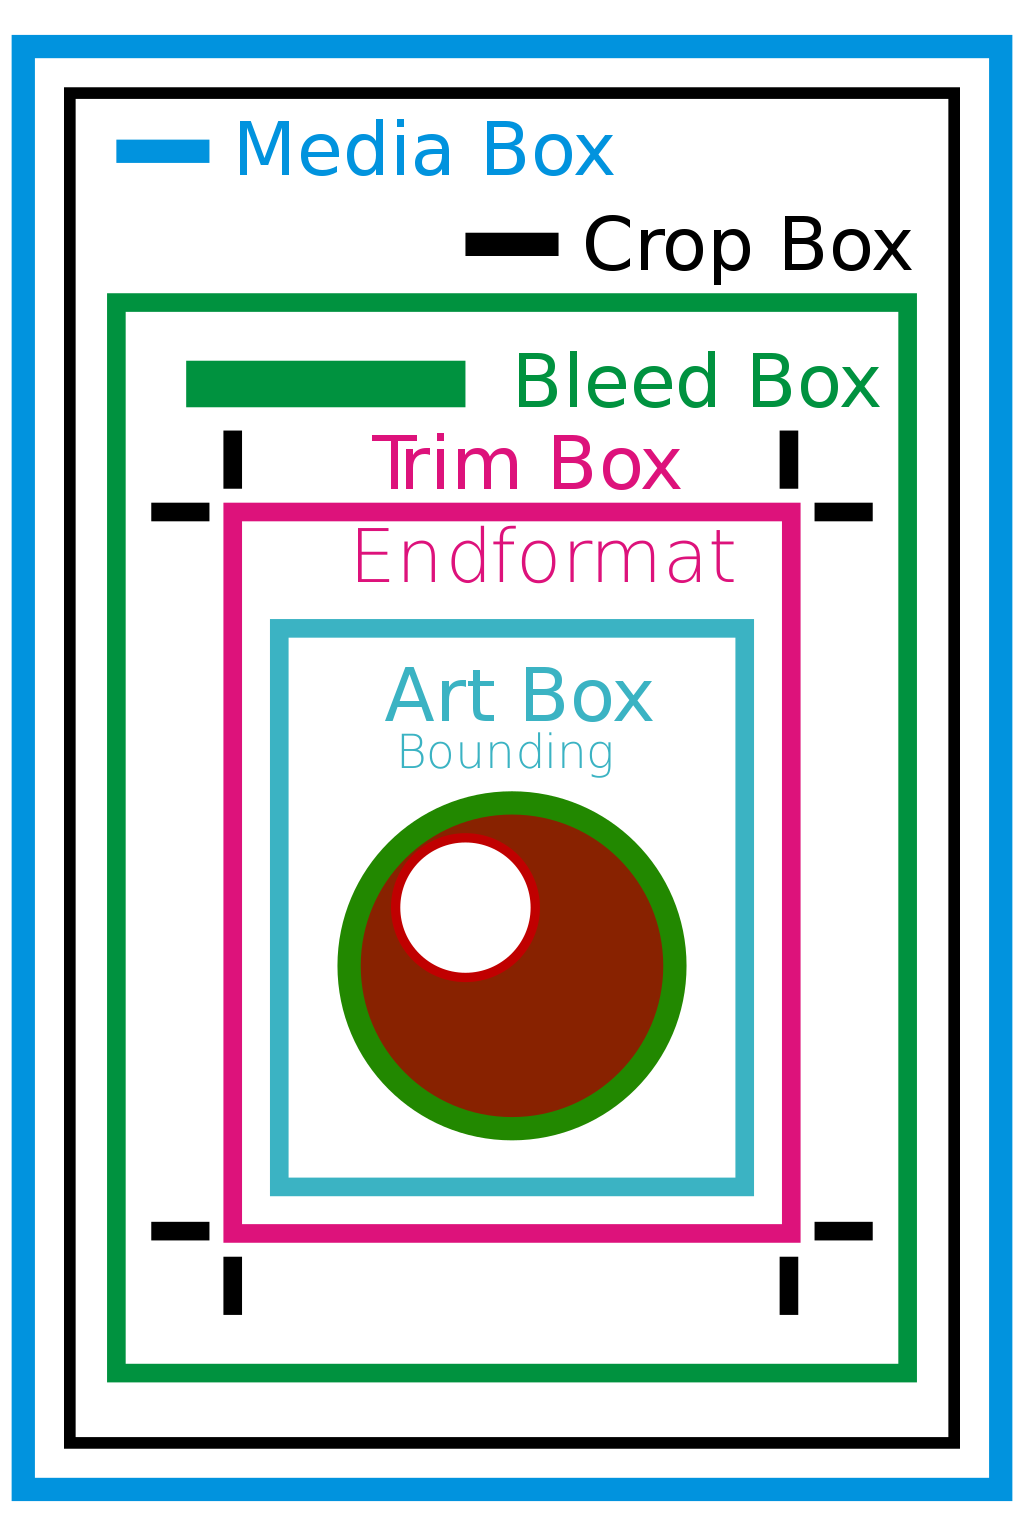
\includegraphics[width=0.6\textwidth]{"images/boxen-wiki-pdf-de.png"}
	\caption{verschachtelte PDF-Boxen \cite{wiki-pdf-de}}
	\label{fig:boxen}
\end{figure}

Erstellt man eine PDF-Datei muss man zwischen composite oder separiert wählen. Bei einer separierten Ausgabe gibt es für jeden Farbauszug bei CMYK inklusive aller Sonderfarben einen eigenen Farbauszug. Inhalte einer Composite-PDF-Datei können einfach verändert werden. Farbsimulationen und die Nutzung der Überdruckvorschau sind in einem separierten PDF-Dokument nicht mehr möglich. Separierte PDF-Dateien sind nicht medienneutral, da eine Farbverrechnung bei der Separation erfolgt. Überfüllung bleibt im Composite-PDF nicht erhalten, jedoch Überdrucken und Aussparen. In modernen Workflows der Druckindustrie hat man sich vom separierten Workflow abgewendet.
\par
Eine PDF-Datei besitzt 3 verschiedene Layers, womit nicht die optional content layers gemeint sind.  Zunächst enthält die content layer alle druckbaren Objekte, sprich Grafiken, Bilder und Texte. Elemente dieses Layers können ausschließlich mit Acrobat Pro bearbeitet werden. Oberhalb der content layer liegt die enhancement layer. In ihr sind Lesezeichen, Hyperlinks, Thumbnails, digitale Signaturen, Annotationen, Formularfelder und alle Multimedia-Elemente wie Video und Audio abgelegt. Die unsichtbare information layer umfasst alle Basisinformationen zu Schriftdaten, Formularfeldinhalten, Verschlüsselungsinformationen, Querverweistabellen und PDF-spezifische Informationen \cite{schneeberger}. PDF-Layouts können in linearar oder nicht linearer Form aufgebaut sein. Nicht lineare PDFs sind kleiner, aber langsamer und die Seiten sind in der Datei an verschiedenen Stellen. Lineare PDFs sind für den Online-Bereich vorgesehen und werden auf die Festplatte in einer linearen Art und Weise gespeichert. Online-PDF-Viewer können somit die Datei schon anzeigen, bevor sie komplett geladen wurde \cite{fileformat}. 

\subsection{Implementierung von Fonts}
Schriften werden als Konturen (outlines) digital gespeichert und mit Instruktionen (hints) versehen, sodass sie generisch skaliert werden können. Fonts werden in PDF als eigenständige Dateien behandelt und die Darstellung wird durch einen speziellen Font-Interpreter bewerkstelligt. Innerhalb der Datei werden Fonts als Dictionary registriert, worin u.a. Fonttyp als Subtype, PostScript-Name, Verschlüsselung und Schriftklasse (für eine mögliche Ersatzschrift) abgelegt sind. Für jeden verwendeten Font wird ein Font-Descriptor in der Datei hinterlegt. PDF verarbeitet 2 Klassen von Fonttypen: Simple-Fonts und Composite-Fonts. Jede Glyphe im Dokument wird über einen Character-Code prozessiert. Daraufhin erfolgt eine Zuordnung des Character Codes zum hinterlegten Encoding (Mapping). Zuletzt wird die Glyphe im aktuellen Font über die Glyphen-ID zum Zeichen der Glyphe aufgerufen. Folglich erzielt das Mapping des Codes und der Aufruf der Glyphe die benötigte Konturbeschreibung. Ein optionales Unicode-Mapping ToUnicode ist von Nöten, damit die Glyphen auch über Unicode verarbeitet werden kann. Ist dieses Mapping nicht vorhanden, so kann keine Textsuche und das Kopieren von Text stattfinden. Fehler im Mapping oder Modifikation von Schriften können zu falsche Ausgabebuchstaben, mangelnde Wiederverwendung und fehlerhafte Textkonvertierung führen. \\
Eine Font-Einbettung kann als zweite Option als Object-Stream gespeichert werden bzw. können Fonts sich auf eine externe Referenz beziehen. Die Beschreibung von Glypen ist bei eingebettete Schriften als Steam im Eintrag FontFile registriert. Falls die Schrift nicht eingebettet wurde, fehlt dieser Eintrag. Schriftsubstitution findet immer dann statt, wenn der Character Code nicht mit der Encoding-Tabelle übereinstimmt. Häufig fehlen bestimmte Glypen im Font. Falls eine Outline-Beschreibung des Fonts zum Erstellungszeitpunkt nicht verfügbar ist, wird die Einbettung des Fonts verhindert. Dies kommt vor allem dann vor, wenn ein Font ein Schutzflag besitzt. Weitere Probleme bei der Schrifteinbettung sind u.a. Laufweitenfehler in Schriften, Fehler in der Buchstabenbeschreibung oder beim Cachen von Fonts. Zwecks der Schriftsubstitution müssen folgende allgemeine Informationen zu einem Font in der PDF-Datei gespeichert sein: Name der Schrift, Fontfamilie, Typ, Subtyp, Schriftstärke (font weight), Zeichenbreite, Laufweite, maximale Ausprägung der FontBox, Dickteninformationen, Positionsangaben über Versal- und x-Höhe und Winkel für Italic (kursiv). Diese Informationen sind selbst bei nicht eingebetteten Schriften vorhanden \cite{schneeberger}. 